\section{Wavelets}

\subsection{Transformadas de sequências finitas}
\begin{frame}%[allowframebreaks]
  \frametitle{Transformadas}
  Seja $\{\phi_k\}_{k \in Z}$ uma base para um subespaço, então qualquer
  função (ou sequência) neste subespaço pode ser escrita como uma combinação
  linear de elementos desta base:
  \begin{equation}
        x = \sum_k a_k \phi_k \ ,
  \end{equation}  
  onde os coeficientes $a_k$ são dados por
  \begin{equation}
        a_k = \langle x , \phi_k \rangle \ .
  \end{equation}
\end{frame}

\begin{frame}%[allowframebreaks]
  \frametitle{Transformadas de Tamanho Finito}
  As Transformadas de Tamanho Finito são representadas da seguinte forma:
  \begin{equation}
  A[k] = \sum_{n=0}^{N-1} x[n] \overline{\phi_k[n]}
  \label{eq:fltransform}
  \end{equation}
  \begin{equation}
        x[n] = \frac{1}{N} \sum_{k=0}^{N-1} A[k] \phi_k [n]
  \label{eq:ifltransform}
  \end{equation}
  
   O exemplo mais comum é a DFT.
   Para a DFT as sequências de base são exponenciais complexas $e^{j2\pi kn/N}$.
\end{frame}

\subsection{Espaço $L^2(\mathbb{R})$}
\begin{frame}%[allowframebreaks]
  \frametitle{Espaço $L^2(\mathbb{R})$}
  $L^p(\mathbb{R})$ é o espaço das funções $f$ definidas em $\mathbb{R}$, assumindo
  valor em $\mathbb{R}$ ou $\mathbb{C}$, tais que
  \begin{equation}
        \Vert f \Vert_p \equiv \left( \int_{-\infty}^{+\infty} \vert f(x) \vert^p \mathrm{d}x \right)^{\frac{1}{p}} < \infty \ .
  \end{equation}
  
  Para $p=2$, definimos o produto interno entre duas funções como
  \begin{equation}
        \langle f,g \rangle = \int_{-\infty}^{\infty} f(x) \overline{g(x)} \mathrm{d}x \ .
  \end{equation}
  $f$ e $g$ são ortogonais se $\langle f,g \rangle = 0$.
\end{frame}

\subsection{Definição}
\begin{frame}%[allowframebreaks]
  Uma função $\psi(x)$ é uma wavelet se $\psi \in L^1(\mathbb{R}) \cap L^2(\mathbb{R})$
  e for tal que a família de funções
  \begin{equation}
        \psi_{j,k} (x) = 2^{-j/2} \psi(2^{-j} x - k) \ ,
  \end{equation}
  onde $j,k \in \mathbb{Z}$, forme uma base para $L^2(\mathbb{R})$.
\end{frame}

\begin{frame}[allowframebreaks]
  \frametitle{Wavelet de Haar}
  A wavelet de Haar é dada por
  \begin{equation}
        \psi(x) = \begin{cases} 1 \quad & \textmd{, se } x \in [0,\frac{1}{2}) ,\\
         -1 \quad & \textmd{, se } x \in [\frac{1}{2},1) ,\\
     0 &  \textmd{, caso contrário.} \end{cases}
  \end{equation}

  \framebreak 

  \begin{columns}[c]
  \column{.33\textwidth}
  \begin{figure}[htp]
  \centering
  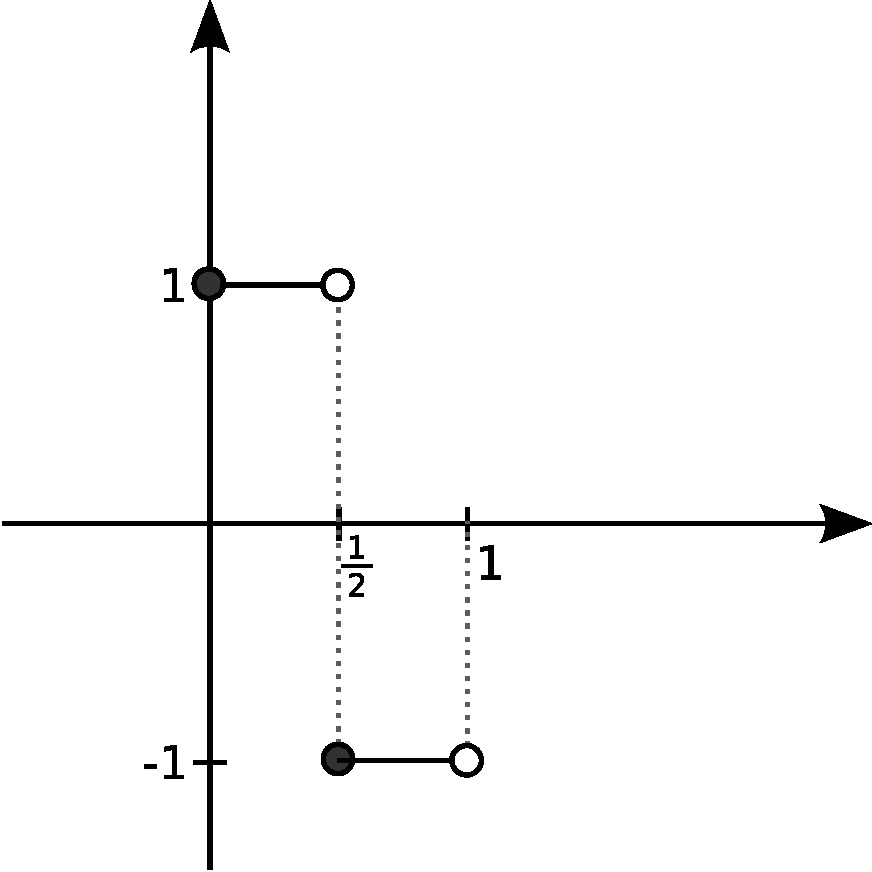
\includegraphics[width=0.9\textwidth]{images/haar_00.pdf}
  \caption{Wavelet de Haar ($\phi(x) = \psi_{0,0}(x)$)}
  \label{fig-haar_00}
  \end{figure}

  \column{.33\textwidth}

  \begin{figure}[htp]
  \centering
  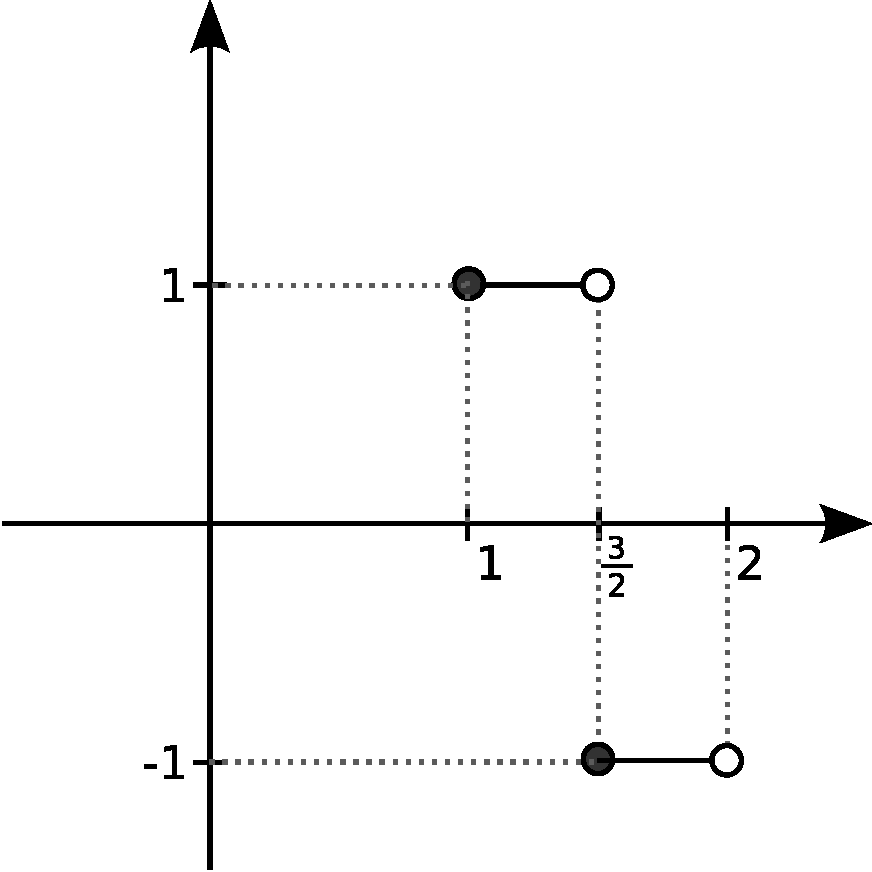
\includegraphics[width=0.9\textwidth]{images/haar_01.pdf}
  \caption{Wavelet de Haar $\psi_{0,1}(x)$}
  \label{fig-haar_01}
  \end{figure}

  \column{.33\textwidth}

  \begin{figure}[htp]
  \centering
  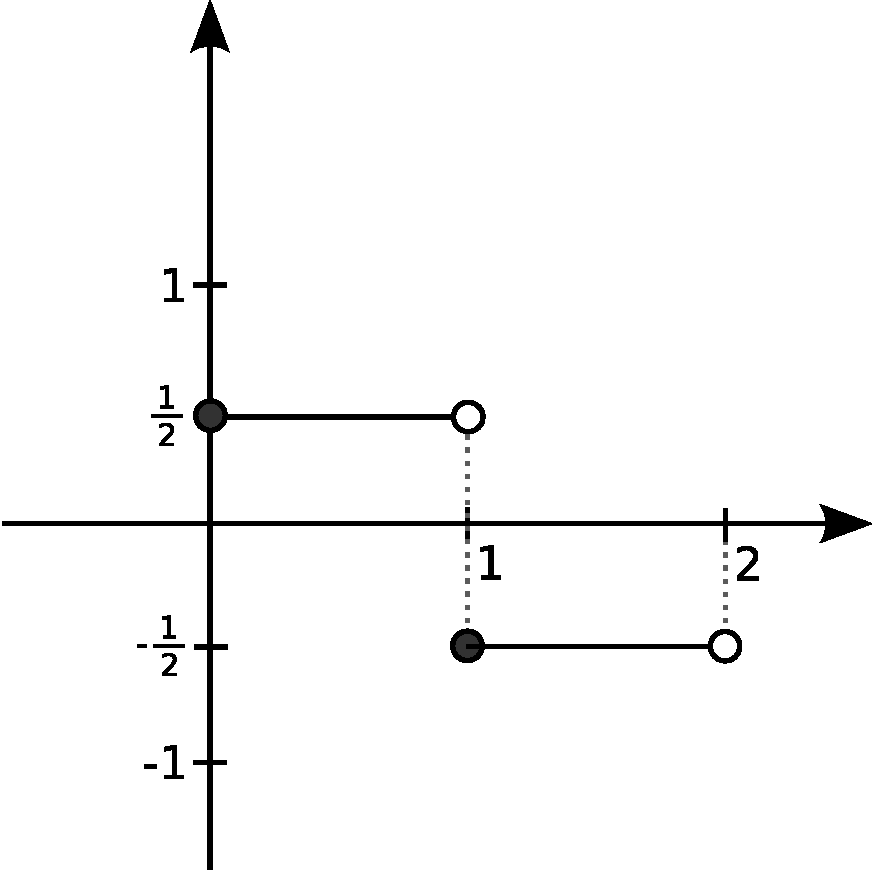
\includegraphics[width=0.9\textwidth]{images/haar_10.pdf}
  \caption{Wavelet de Haar: $\psi_{1,0}(x)$}
  \label{fig-haar_10}
  \end{figure}

  \end{columns}
\end{frame}


\begin{frame}[allowframebreaks]
  \frametitle{Função Escala}
  Às funções wavelet $\psi$ existem associadas as funções escala $\phi$.
  Existe a seguinte relação entre elas:
  \begin{equation}
        \phi(x) = \sqrt{2} \sum_k h_k \phi(2x -k)
  \end{equation}
  \begin{equation}
        \psi(x) = \sqrt{2} \sum_k g_k \phi(2x -k)
  \end{equation}
  Os coeficientes $h_k$ e $g_k$ são os coeficientes de filtro associados 
  à wavelet e à função escala, respectivamente.

  No caso das wavelets de suporte compacto, apenas um número finito de valores
  desses coeficientes serão diferentes de zero (filtro FIR). 

  \framebreak 

  Para o casa da wavelet de Haar, teremos a seguinte relação:
  \begin{equation}
  \phi(x) = \phi(2x) + \phi(2x - 1)
  \end{equation}
  \begin{equation}
  \psi(x) = \phi(2x) - \phi(2x - 1)
  \end{equation}

  A função escala associada à wavelet de Haar é dada por
  \begin{columns}[c]
  \column{.5\textwidth}
    \begin{equation}
        \phi(x) = \begin{cases} 1 \quad & , 0 \leq x < 1 ,\\
     0 &  \textmd{, caso contrário.} \end{cases}
    \end{equation}
  \column{.5\textwidth}
    \begin{figure}[htp]
    \centering
    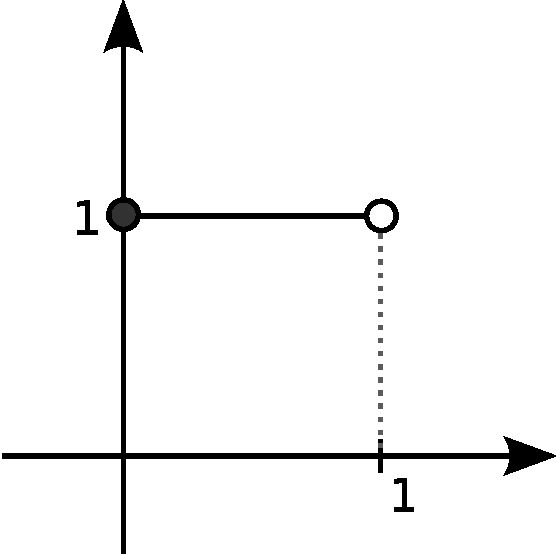
\includegraphics[width=0.5\textwidth]{images/haar_escala_00.pdf}
    \caption{$\phi(x) = \phi_{0,0}(x)$}
    \label{fig-haar_escala_00}
    \end{figure}
  \end{columns} 
\end{frame}

\begin{frame}[allowframebreaks]
  \frametitle{Exemplo}
    \begin{figure}[htp]
    \centering
    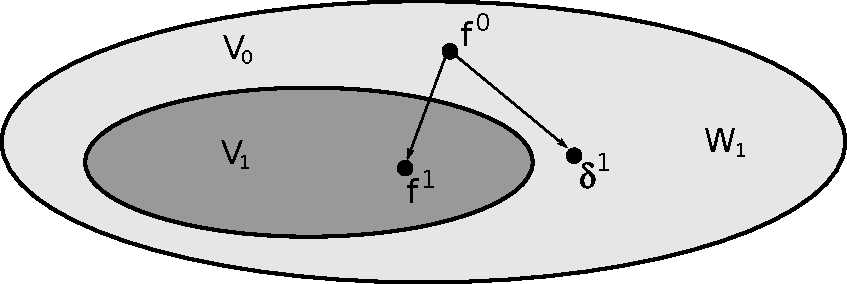
\includegraphics[width=0.5\textwidth]{images/fun_f0_d.pdf}
    \caption{Decomposição de uma função: $f^0 = f^1 + \delta^1$ \citep{araujo2007}.}
    \label{fig-funf1}
    \end{figure}

    \framebreak

    \begin{figure}[htp]
    \centering
    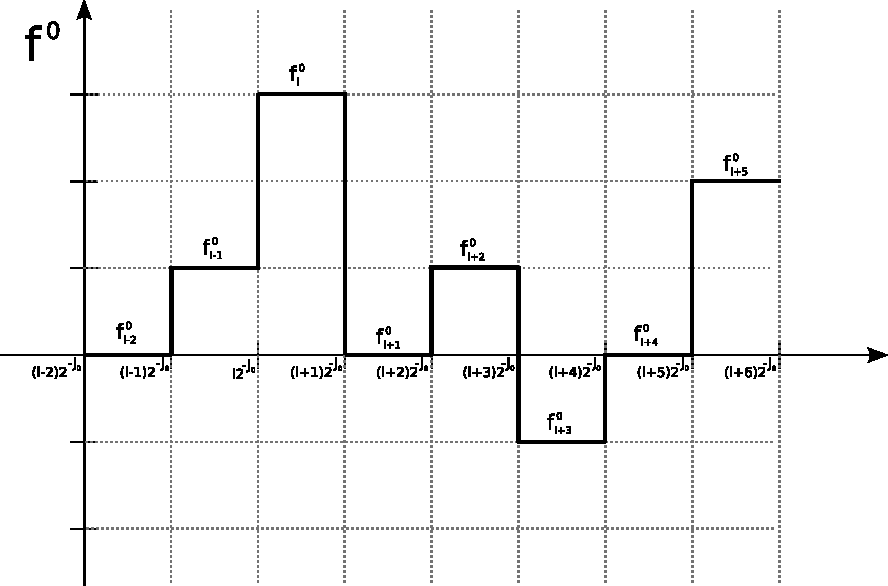
\includegraphics[width=0.5\textwidth]{images/fun_f0_1.pdf}
    \caption{Decomposição de uma função: $f^0 = f^1 + \delta^1$ \citep{araujo2007}.}
    \label{fig-funf1}
    \end{figure}

    \framebreak

    \begin{figure}[htp]
    \centering
    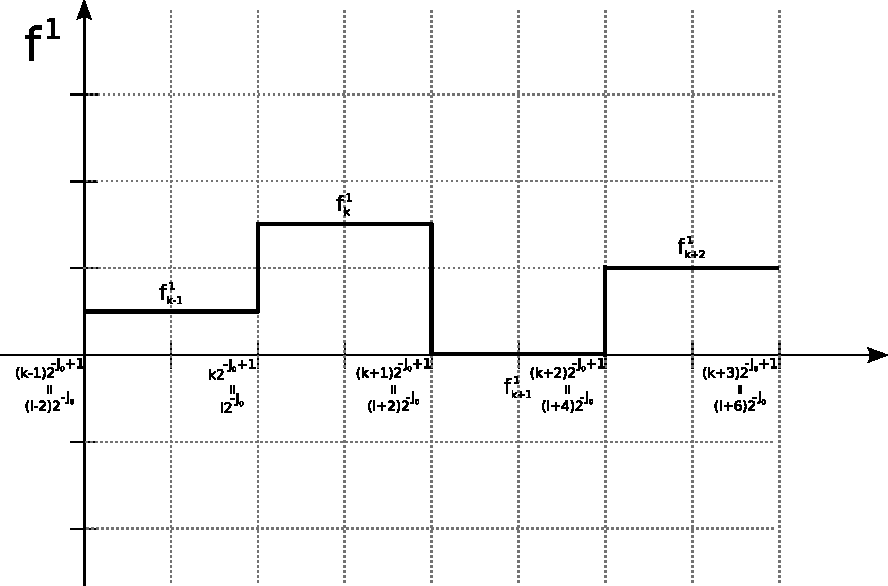
\includegraphics[width=0.5\textwidth]{images/fun_f0_2.pdf}
    \caption{Decomposição de uma função: $f^0 = f^1 + \delta^1$ \citep{araujo2007}.}
    \label{fig-funf2}
    \end{figure}

    \framebreak

    \begin{figure}[htp]
    \centering
    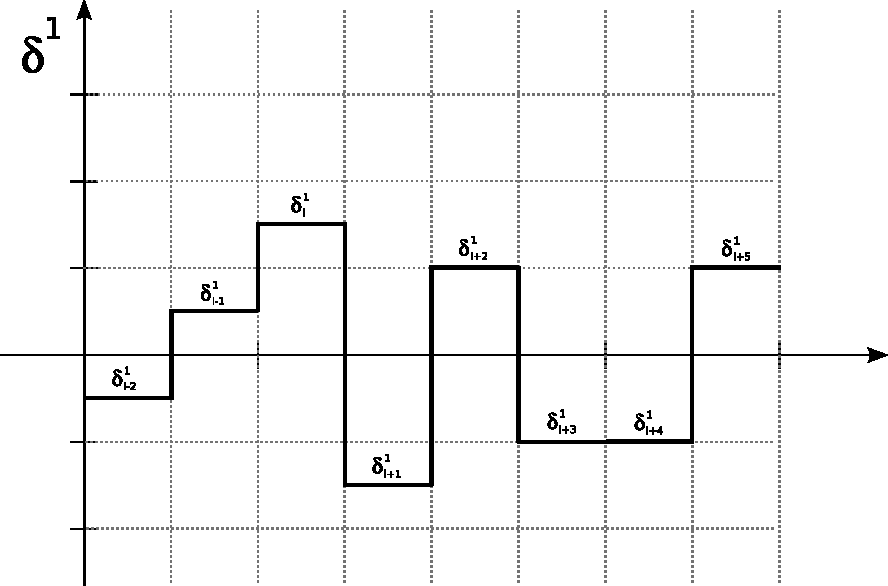
\includegraphics[width=0.5\textwidth]{images/fun_f0_3.pdf}
    \caption{Decomposição de uma função: $f^0 = f^1 + \delta^1$ \citep{araujo2007}.}
    \label{fig-funf3}
    \end{figure} 

    \framebreak

    \begin{figure}[htp]
    \centering
    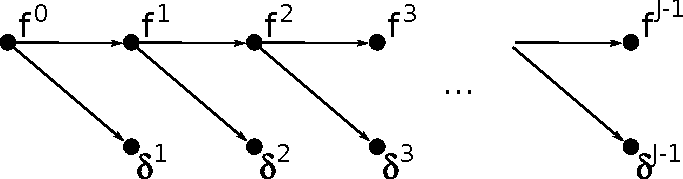
\includegraphics[width=0.5\textwidth]{images/fun_f0_d2.pdf}
    \caption{Decomposição de uma função: $f^0 = f^1 + \delta^1 = f^2 + \delta^2 + \delta^1 = \ldots f^{J-1} + \sum_{j=1}^{J-1} \delta^j$ \citep{araujo2007}.}
    \label{fig-funf4}
    \end{figure}

\end{frame}

\begin{frame}%[allowframebreaks]
  \frametitle{Algoritmo Rápido de Decomposição}
  Temos o seguinte algoritmo em cascata para calcular os coeficientes de wavelet
  $\{d_{j,n}\}$
  
  \begin{equation}
     \begin{matrix}
        a_{j_0,.} & \rightarrow & a_{j_0+1,.} & \rightarrow & a_{j_0+2,.} & \ldots & a_{j_0+J-1,.} & \rightarrow  & a_{j_0+J,.} \\
                  & \searrow & d_{j_0+1,.} & \searrow & d_{j_0+2,.} & \ldots & & \searrow & d_{j_0+J,.}
     \end{matrix}
  \end{equation}

  Os coeficientes são calculados através da seguintes relações:
  \begin{equation}
        a_{j,n} = \sum_k \overline{h_k} a_{j-1,2n+k} \textmd{ , e}
  \end{equation}
  \begin{equation}
        d_{j,n} = \sum_k \overline{g_k} a_{j-1,2n+k} \textmd{ .}
  \end{equation}
\end{frame}

\begin{frame}%[allowframebreaks]
  \frametitle{Algoritmo Rápido de Reconstrução}

  O algoritmo em cascata para reconstruir um sinal é representado abaixo:
  \begin{equation}
     \begin{matrix}
        a_{j_0+J,.} & \rightarrow & a_{j_0+J-1,.} & \rightarrow & \ldots & a_{j_0+1,.} & \rightarrow  & a_{j_0,.} \\
        d_{j_0+J,.} & \nearrow & d_{j_0+J-1,.} &   &   \ldots & d_{j_0+1,.} & \nearrow & 
     \end{matrix}
  \end{equation}

  e descrito pela seguinte relação
  \begin{equation}
        a_{j-1,n} = \sum_k \overline{h_{n-2k}} a_{j,k}  + \sum_k \overline{g_{n-2k}} d_{j,k} \textmd{ .}
  \end{equation}
\end{frame}

\begin{frame}%[allowframebreaks]
  \frametitle{Algoritmo - Equivalência}

  No algoritmo de decomposição, temos a seguinte relação
  \begin{equation}
  \langle f, \phi_{j,k} \rangle = \sum_{n} \overline{h_{n-2k}} \langle f, \phi_{j-1,n} \rangle ,
  \label{eq:algoritmo_rapido_mudanca_escala_1}
  \end{equation}
  \begin{equation}
  \langle f, \psi_{j,k} \rangle = \sum_{n} \overline{g_{n-2k}} \langle f, \psi_{j-1,n} \rangle .
  \label{eq:algoritmo_rapido_mudanca_escala_2}
  \end{equation}

  Isso equivalente a fazer
  \begin{equation}
  \langle f, \phi_{j,k} \rangle = (\downarrow 2) \left( \langle f, \phi_{j-1,n} \rangle \ast \overline{h_{-n}} \right)
  \label{eq:algoritmo_rapido_mudanca_escala_1a}
  \end{equation}
  \begin{equation}
  \langle f, \psi_{j,k} \rangle = (\downarrow 2) \left( \langle f, \psi_{j-1,n} \rangle \ast \overline{g_{-n}} \right) 
  \textmd{ . }
  \label{eq:algoritmo_rapido_mudanca_escala_2a}
  \end{equation}

  Estas equações podem ser reescritas na forma matricial.
\end{frame}

\begin{frame}[allowframebreaks]
  \frametitle{Algoritmo - Forma Matricial}
  
  \begin{itemize}
        \item $H$ e $G$ são as matrizes dos filtros $h$ e $g$, respectivamente
        \item $D$ é a matriz de \emph{downsample}
  \end{itemize}

  \begin{columns}[c]
  \column{.5\textwidth}
  \begin{equation}
  H =
    \begin{bmatrix}
    .   &     &     &     &    \\
    h_0 & h_1 &     &     &    \\
        & h_0 & h_1 &     &    \\
        &     & h_0 & h_1 &    \\
        &     &     & .   & .  \\
  \end{bmatrix}
  \label{eq:filtragem_matricial}
  \end{equation}

  \column{.5\textwidth}
  \begin{equation}
  D =
  \begin{bmatrix}
  .   &     &     &     &     &     &     &    \\
  1   &  0  &     &     &     &     &     &    \\
      &     &  1  &  0  &     &     &     &    \\
      &     &     &     &  1  &  0  &     &    \\
      &     &     &     &     &     &  .  & .  \\
  \end{bmatrix}
  \label{eq:matriz_decimacao_2}
  \end{equation}
  \end{columns}


  \framebreak
  
  \begin{equation}
  DH =
  \begin{bmatrix}
  .   &     &     &     &     &     &      &    \\
  h_0 & h_1 &     &     &     &     &      &    \\
      &     & h_0 & h_1 &     &     &      &    \\
      &     &     &     & h_0 & h_1 &      &    \\
      &     &     &     &     &     &  .   & .  \\
  \end{bmatrix}
  \label{eq:filtragem_matricial}
  \end{equation}

  \begin{equation}
  a_j = \begin{bmatrix} \vdots \\ a_{j,-1} \\ a_{j,0} \\ a_{j,1} \\ \vdots \\ \end{bmatrix} \textmd{.}
  \end{equation}

  \framebreak

  As operações escritas em (\ref{eq:algoritmo_rapido_mudanca_escala_1a}) e
  (\ref{eq:algoritmo_rapido_mudanca_escala_2a}) podem ser representadas então por:
  \begin{equation}
  a_{j} = D H a_{j-1} \textmd{,}
  \end{equation}
  \begin{equation}
  d_{j} = D G a_{j-1} \textmd{.}
  \end{equation}


  \begin{figure}[hptb]
  \centering
  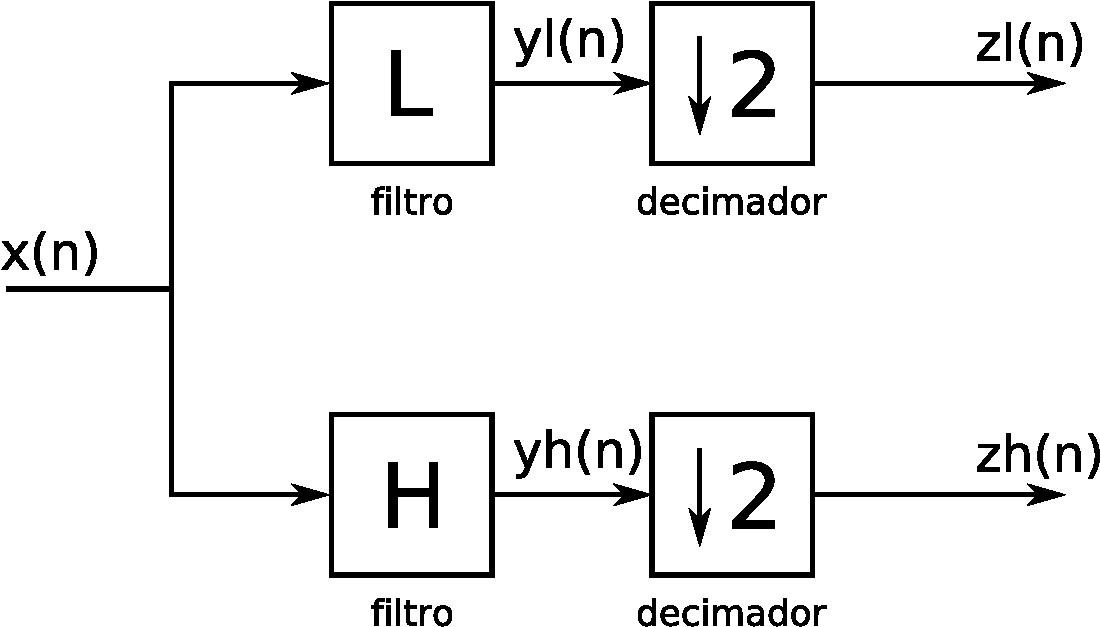
\includegraphics[width=.3\textwidth]{images/banco_filtros.pdf}
  \caption{Banco de Filtros.}
  \label{fig:banco_filtros}
  \end{figure}

\end{frame}


\subsection{Banco de Filtros}
\begin{frame}[allowframebreaks]
  \frametitle{Banco de Filtros}
  \begin{figure}[hptb]
  \centering
  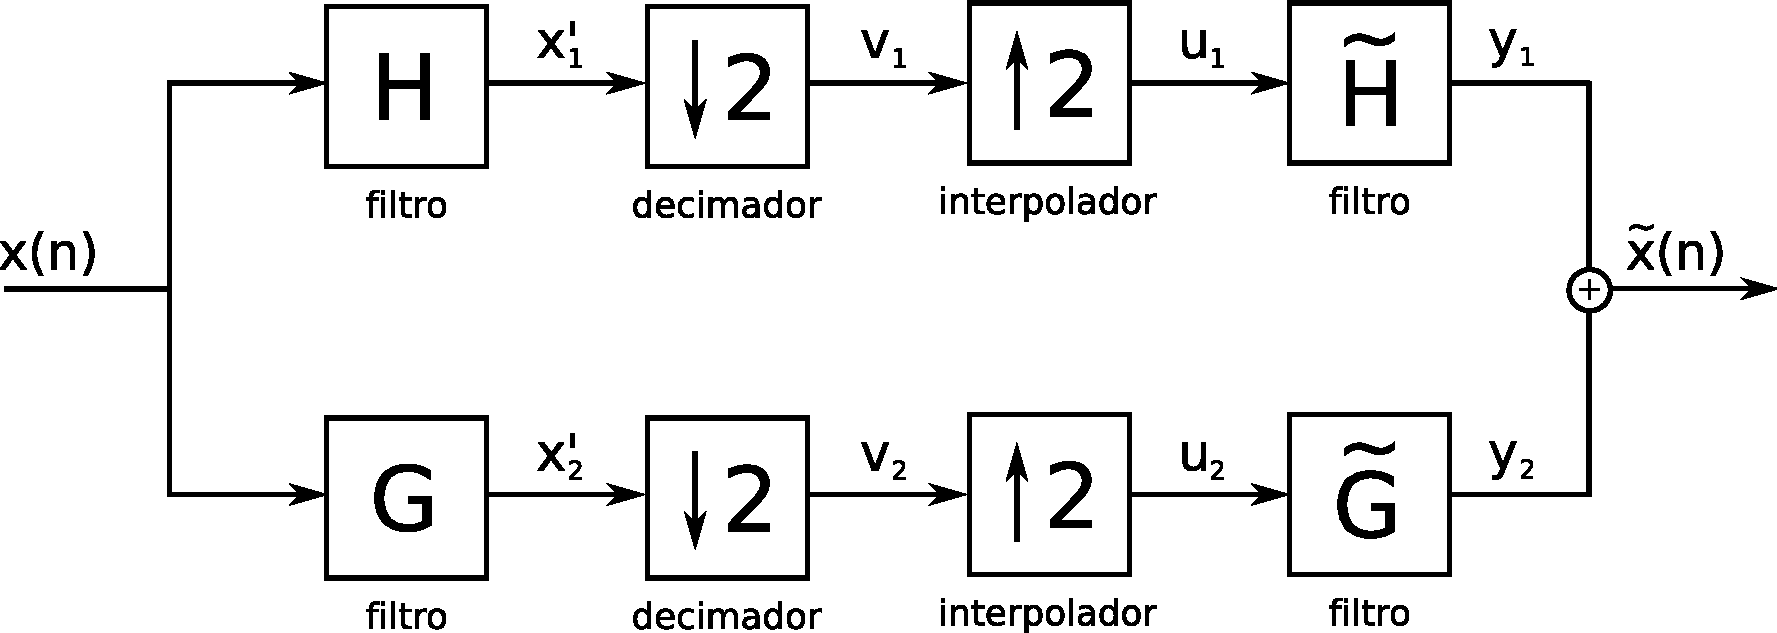
\includegraphics[width=.75\textwidth]{images/banco_filtros_comp.pdf}
  \caption{Banco de Filtros (decomposição e síntese).}
  \label{fig:filter_bank_complete}
  \end{figure}

  \framebreak

  \begin{figure}[hptb]
  \centering
  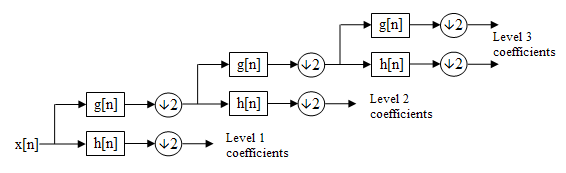
\includegraphics[width=.75\textwidth]{images/wavelets_filter_bank.png}
  \caption{Banco de Filtros: decomposição (Wikipedia).}
  \label{fig:filter_bank_dec}
  \end{figure}

  \framebreak

  \begin{figure}[hptb]
  \centering
  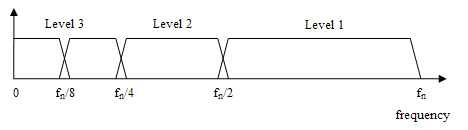
\includegraphics[width=.75\textwidth]{images/wavelets_filterbank_freq.png}
  \caption{Banco de Filtros Wavelets no Domínio da Frequência (Wikipedia).}
  \label{fig:wavelets_filterbank_freq}
  \end{figure}

  \framebreak

  \begin{figure}[hptb]
  \centering
  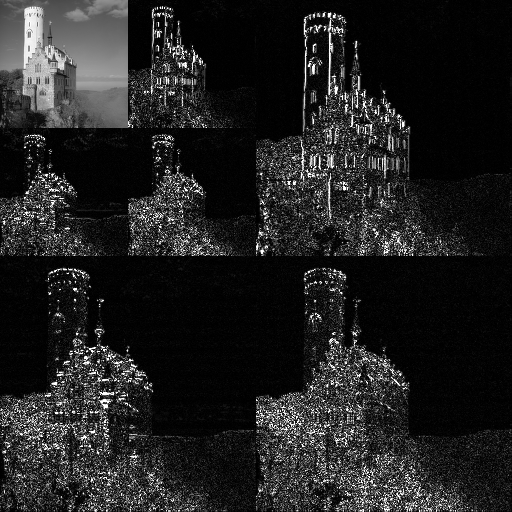
\includegraphics[width=.5\textwidth]{images/wavelet_lichtenstein.png}
  \caption{JPEG200: duas etapas da decomposição wavelet 2D da foto do castelo de Lichtenstein.}
  \label{fig:wlichtenstein}
  \end{figure}

\end{frame}






\subsection{Incerteza de Heisenberg}
\begin{frame}[allowframebreaks]
  \frametitle{Princípio da Incerteza de Heisenberg}
  Um par de variáveis observáveis \textbf{não} pode ser determinado
  com qualquer precisãoo desejada para ambas as variáveis. 
  Existe um limite para o qual aumentar a precisão em
  uma variável implica em diminuir a precisão na outra. 
  Este limite é estabelecido pela seguinte relação
  entre as variâncias das variáveis
  \begin{equation}
  \sigma_{t}^{2}\sigma_{\omega}^{2} \geq \frac{1}{4} \textmd{ . }
  \label{eq:heisenberg_variancias}
  \end{equation}

  \framebreak

  \begin{figure}[hptb]
  \centering
  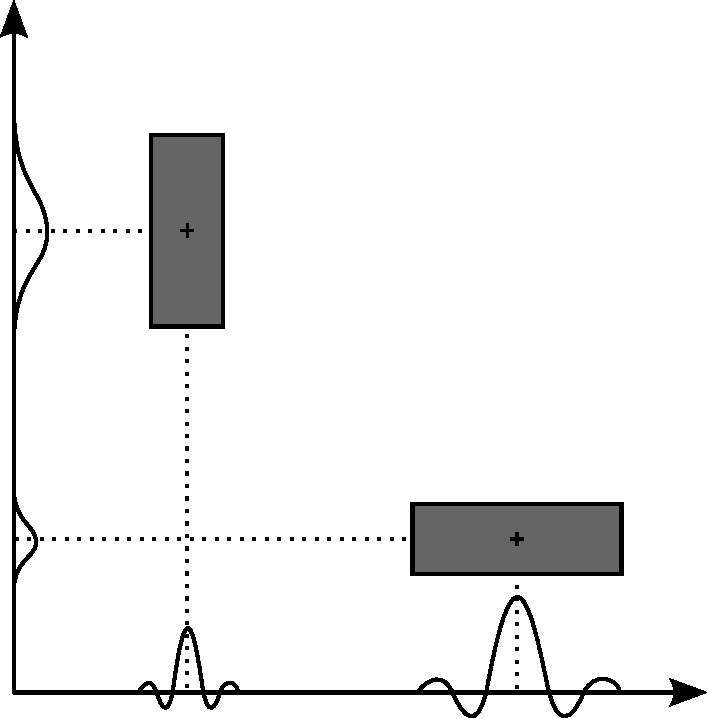
\includegraphics[width=.4\textwidth]{images/time_freq_box.pdf}
  \caption{Caixas Tempo-Frequência \citep{araujo2007}.}
  \label{fig:caixas_tempo-freq}
  \end{figure}

  \framebreak

  \begin{columns}[c]
  \column{.5\textwidth}
  \begin{figure}[hptb]
  \centering
  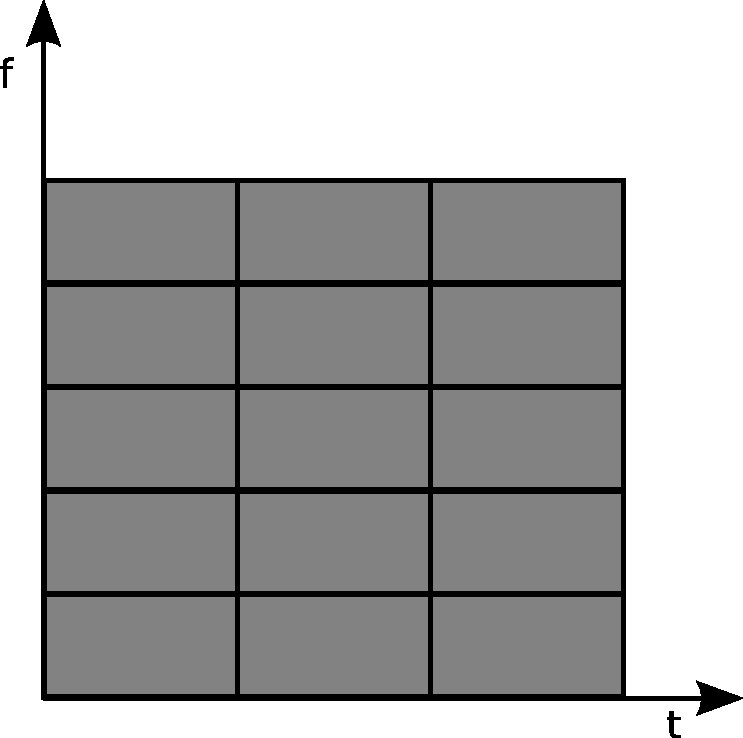
\includegraphics[width=.7\textwidth]{images/heisenber_boxes_fourier_janela.pdf}
  \caption{Caixas de Heisenberg para a transformada Fourier com janela.}
  \label{fig:caixas_tempo-freq_fourier_janela}
  \end{figure}

  \column{.5\textwidth}
  \begin{figure}[hptb]
  \centering
  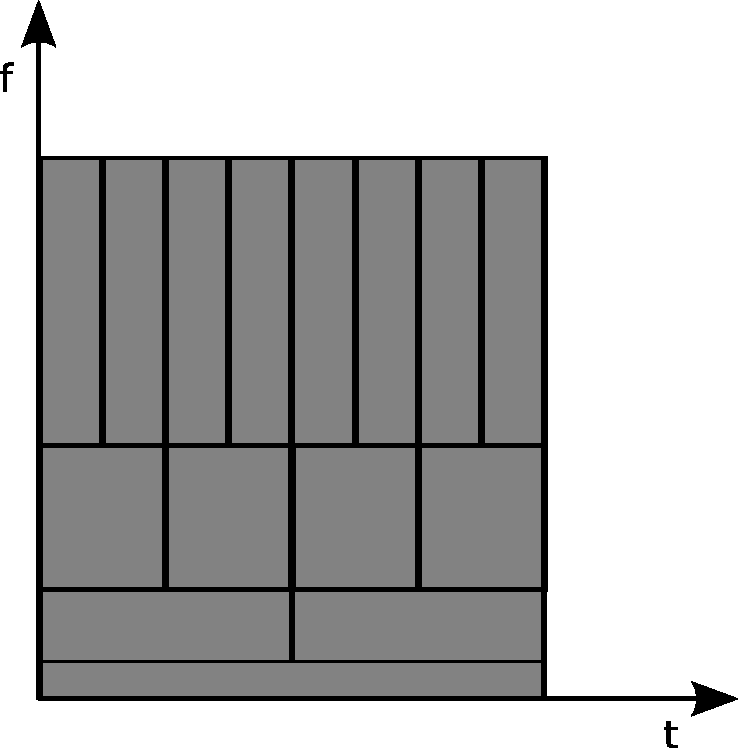
\includegraphics[width=.7\textwidth]{images/heisenber_boxes_wavelet.pdf}
  \caption{Caixas de Heisenberg para a transformada wavelet.}
  \label{fig:caixas_tempo-freq_wavelet}
  \end{figure}
  \end{columns} 
\end{frame}

\subsection{ARM}
\begin{frame}[allowframebreaks]
  \frametitle{Análise em Resoluções Múltiplas (ARM)}
  Diz-se que há uma ARM quando as seguintes propriedades são satisfeitas para 
  uma sequência de subespaços $\{V_j\}_{j \in \mathbb{Z}}$ 
  fechados de $L^2(\mathbb{R})$
  \begin{eqnarray}
  \forall j \in \mathbb{Z} \ , \ V_{j+1} \subset V_{j} \textmd{ , } \label{eq:ARM_1}\\
  \forall (j,k) \in \mathbb{Z}^2 \ , \ f \in V_j \Leftrightarrow f(\cdot - 2^{j}k) \in V_j \textmd{ , } \label{eq:ARM_2}\\
  \forall j \in \mathbb{Z} \ , \ f \in V_j \Leftrightarrow f(2^{j} \cdot) \in V_{0} \textmd{ , } \label{eq:ARM_3}\\
  \lim_{j \rightarrow +\infty} V_j = \bigcap_{j \in \mathbb{Z}} V_j = \{0\} \textmd{ , } \label{eq:ARM_4}\\
  \lim_{j \rightarrow -\infty} V_j = \overline{\bigcup_{j \in \mathbb{Z}} V_j} = L^2(\mathbb{R}) \textmd{ , } \label{eq:ARM_5}\\
  \exists \phi \in V_0 \textmd{ tal que } \phi_{0,k}(t) = \phi(t - k) \textmd{ constitui } \\ \textmd{uma base ortonormal para } V_0 \label{eq:ARM_6} \textmd{.} \nonumber
  \end{eqnarray}

  \framebreak

  Sequência de Subespaços Encaixantes:

  Temos a seguinte relação: $V_j = V_{j+1} \oplus W_{j+1}$
  e também a ortogonalidade entre os subespaços 
  $W_j$ ($W_{j} \bot W{j'}$ quando $j \neq j'$) e entre
  $W_{j}$ e $V_{j'}$ onde $j' \geq j$.
  
  \begin{equation}
  V_{j} = V_{j+1+J} \oplus \bigoplus_{n = j+1}^{j+1+J} W_{n} \textmd{ . }
  \label{eq:sum_subespacos_W}
  \end{equation}
  
  Uma função $f^j$ inicialmente representada em $V^j$ pode ser decomposta 
  como uma versão de baixa resolução $f^{j+1+J}$ somada aos detalhes $\delta^n$
  correspondentes a cada subespaço $W_n$:
  \begin{equation}
  f^j = f^{j+1+J} + \sum_{n = j+1}^{j+1+J} \delta^n \textmd{.}
  \label{eq:decomposicao_funcao_f_J}
  \end{equation}

  \framebreak

  \begin{figure}[hptb]
  \centering
  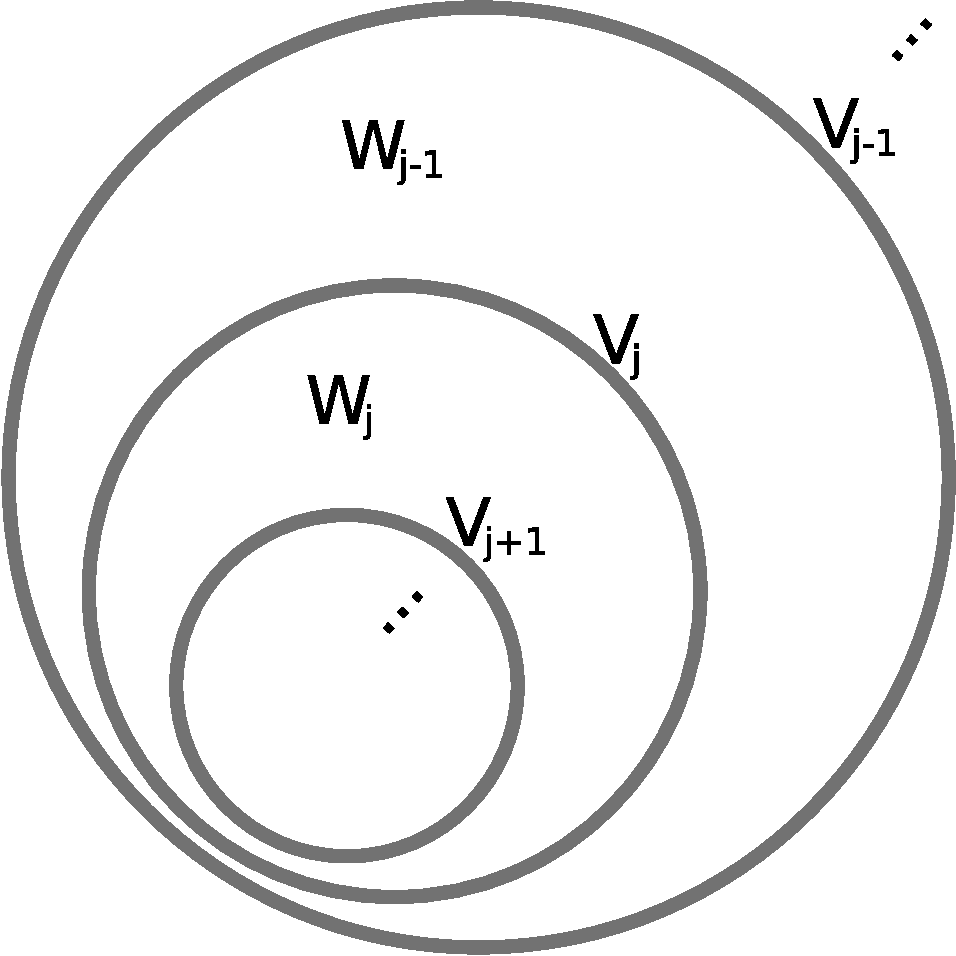
\includegraphics[width=.3\textwidth]{images/subespacos_encaixantes.pdf}
  \caption{Sequencia de subespaços encaixantes.}
  \label{fig:subespacos_encaixantes}
  \end{figure} 

  \framebreak

  Suponha que uma função qualquer $f \in L^2(\mathbb{R})$ 
  possa ser escrita na base $V_{j}$, então
  \begin{equation}
  P_{V_j} f = f^j = \sum_{k} a_{j,k} \phi_{j,k} \textmd{,}
  \label{eq:f_em_Vj}
  \end{equation}
  onde os coeficientes são dados por $a_{j,k} = \langle f, \phi_{j,k} \rangle$.

  \begin{eqnarray}
  a_{j,k} &=& \langle f, \sum_{n} h_n \phi_{j-1,2k+n} \rangle \nonumber \\
          &=& \sum_{n} \overline{h_n} \langle f, \phi_{j-1,2k+n} \rangle \nonumber \\
          &=& \sum_{n} \overline{h_n} a_{j-1,2k+n}
  \label{eq:coef_ajk_reescrito}
  \end{eqnarray}

  \framebreak

  Como $f^{j-1} = f^{j} + \delta^{j}$, onde 
  $f^{j}$ é a projeção sobre o subespaço $V_{j}$ e $\delta_{j}$ a projeção sobre
  $W_{j}$ ($V_{j-1} = V_{j} \oplus W_{j}$), temos
  \begin{equation}
  \delta^j = \sum_k d_{j,k} \psi_{j,k}
  \label{eq:funcao_delta_detalhe}
  \end{equation}
  onde $d_{j,k} = \langle f, \psi_{j,k} \rangle$.
  \begin{eqnarray}
  d_{j,k} &=& \langle f, \sum_{n} g_n \phi_{j-1,2k+n} \rangle \nonumber \\
        &=& \sum_{n} \overline{g_n} \langle f, \phi_{j-1,2k+n} \rangle \nonumber \\
        &=& \sum_{n} \overline{g_n} a_{j-1,2k+n} \textmd{.}
  \label{eq:coef_djk_ajk}
  \end{eqnarray}

\end{frame} 


\subsection{Famílias de Wavelets}

\begin{frame}[allowframebreaks]
   \frametitle{Algumas Famílias de Wavelets}
   Haar, Daubechies, Symlets, Coiflets, BiorSplines,
   ReverseBior, Meyer, DMeyer, Gaussian, Mexican hat,
   Morlet, Complex Gaussian, Shannon, Frequency B-Spline,
   Complex Morlet, etc.

   \framebreak

  \begin{figure}[hptb]
  \centering
  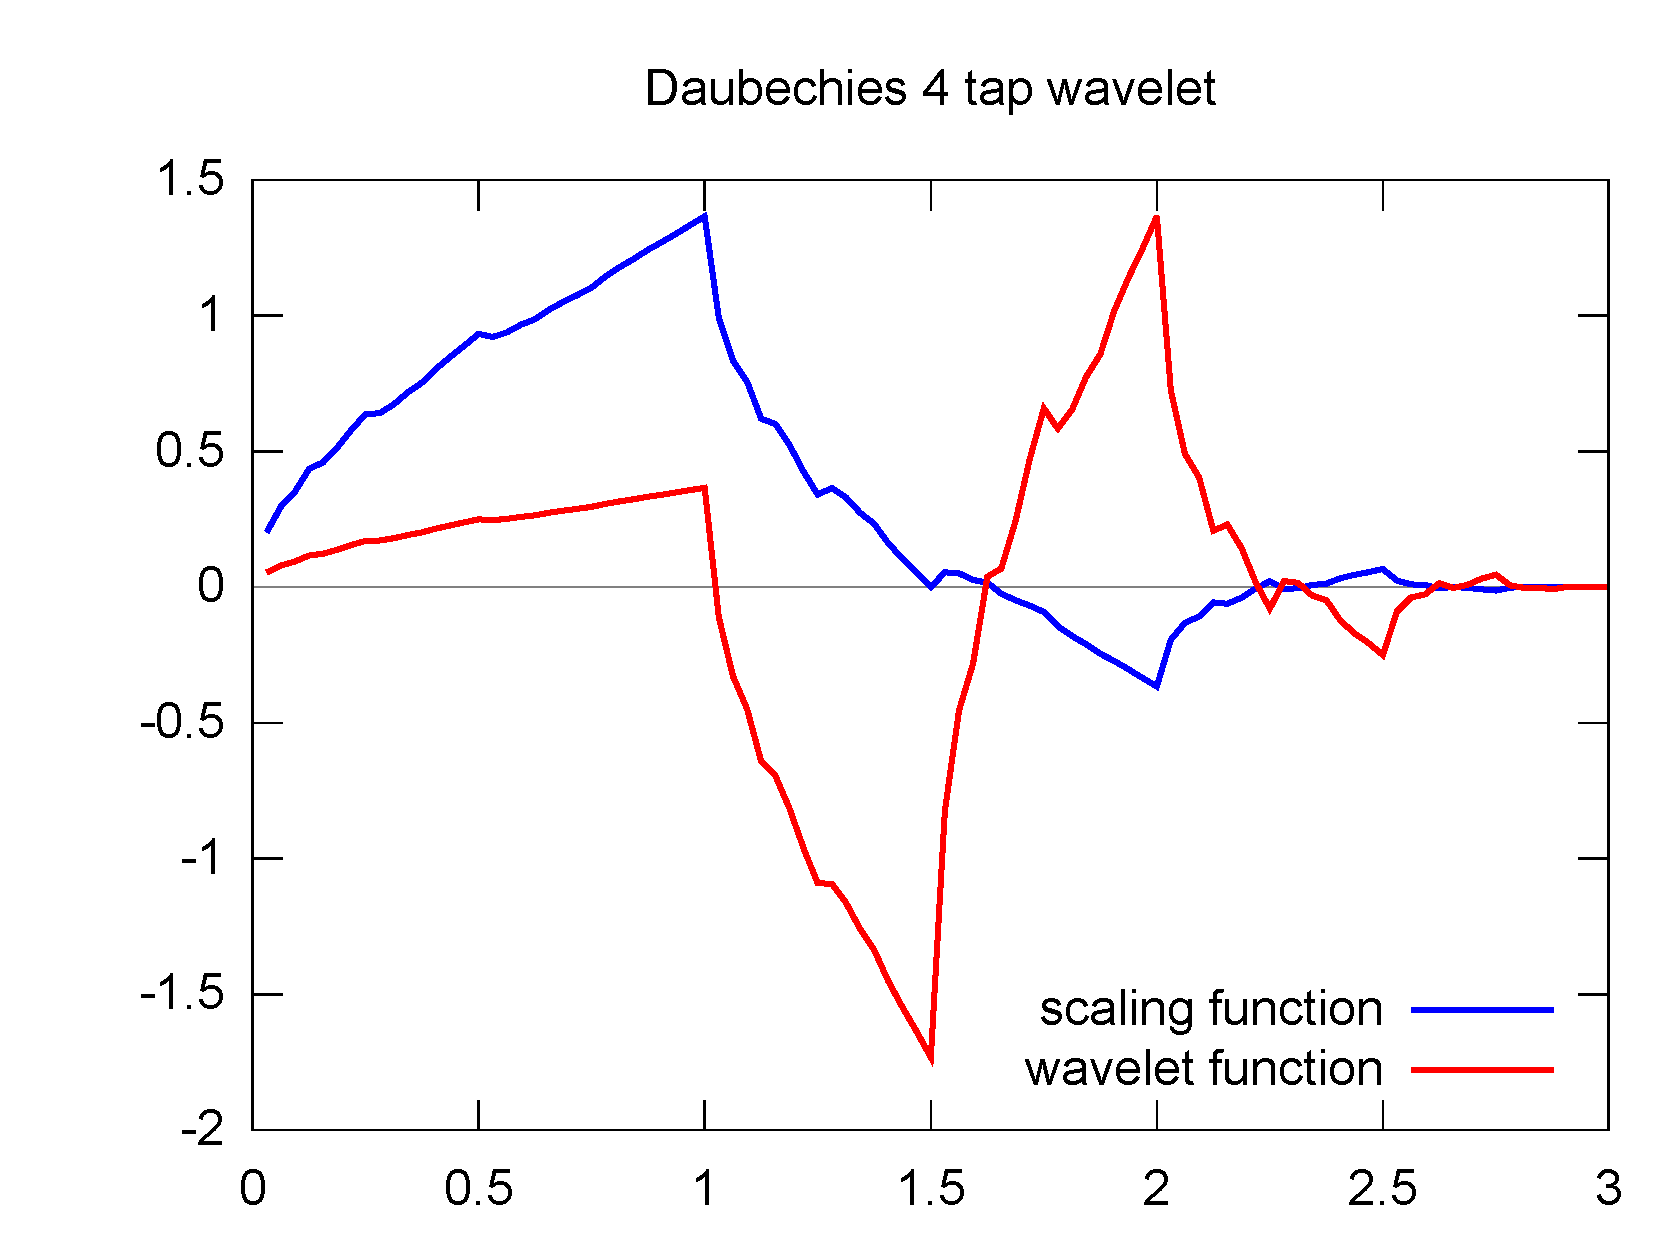
\includegraphics[width=.5\textwidth]{images/db4.pdf}
  \caption{Wavelet de Daubechies 4.}
  \label{fig:db4}
  \end{figure} 

  \framebreak

 \begin{columns}[T]
 \column{.33\textwidth}
  \begin{figure}[hptb]
  \centering
  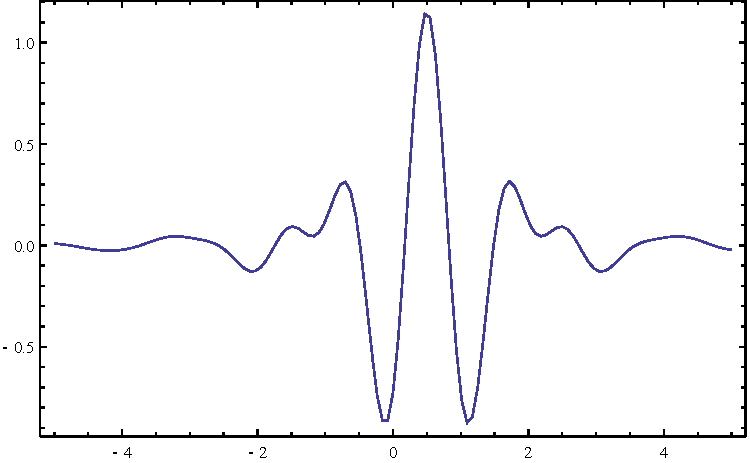
\includegraphics[width=.9\textwidth]{images/meyer.pdf}
  \caption{Wavelet de Meyer.}
  \label{fig:meyer}
  \end{figure} 
 \column{.33\textwidth}
  \begin{figure}[hptb]
  \centering
  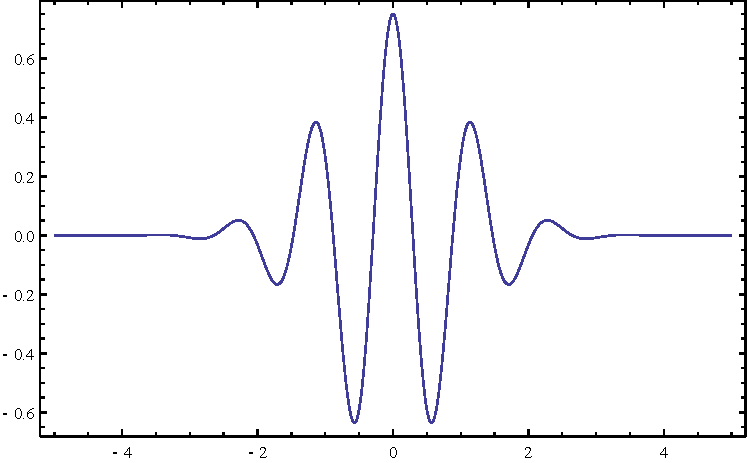
\includegraphics[width=.9\textwidth]{images/morlet.pdf}
  \caption{Wavelet de Morlet.}
  \label{fig:morlet}
  \end{figure} 
 \column{.33\textwidth}
  \begin{figure}[hptb]
  \centering
  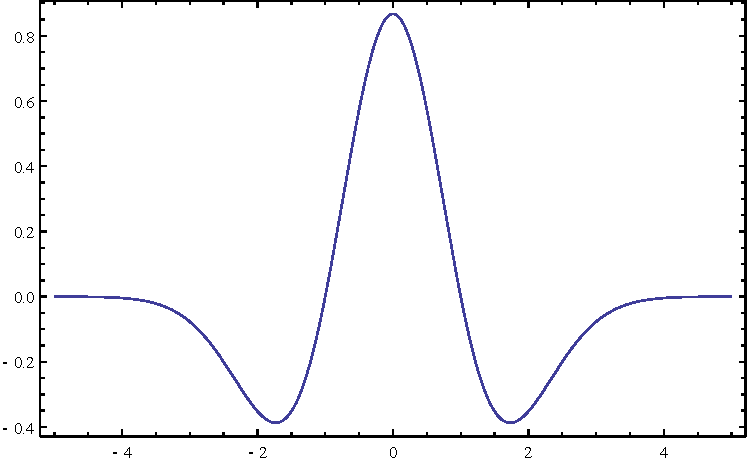
\includegraphics[width=.9\textwidth]{images/mexicanhat.pdf}
  \caption{Wavelet Chapéu Mexicano.}
  \label{fig:mexicanhat}
  \end{figure} 
 \end{columns}

\end{frame}

\begin{frame}[allowframebreaks]
  \frametitle{Wavelets de Daubechies}
  As wavelets de Daubechies são wavelets que possuem todos os momentos
  até ordem $N-1$ nulos, ou seja,
  \begin{equation}
        \int_{-\infty}^{\infty} x^l \psi(x) \mathrm{d}x = 0 , \quad l = 0, \ldots, N-1.
  \end{equation}
  Observação: quando $l=0$ temos a média, quando $l=1$ a variância, e quando $l=2$ a obliquidade (\emph{skewness}).
  As wavelets de Haar podem ser vitas como um caso particular das wavelets de 
  Daubechies quando $N=1$.
  Para as wavelets de Daubechies, os valores de $h_k$ não nulos serão apenas $2N$
  valores, raízes de equações algébricas, calculadas por métodos numéricos.
  
  \framebreak

  \begin{itemize}
        \item Daub2 (Haar) \\ $h_0 = h_1 = \sqrt{2}/2$ 
        \item Daub4 \\ $h_0 = (1+\sqrt{3})/4\sqrt{2}$, $h_1 = (3+\sqrt{3})/4\sqrt{2}$, $h_2 = (3-\sqrt{3})/4\sqrt{2}$ e $h_3 = (1-\sqrt{3})/4\sqrt{2}$
  \end{itemize}  

\end{frame}
\note{
  Obs.: Compressão de Imagens.
  
  A vantagem em se ter uma wavelet com vários momentos nulos é o fato 
  dos coeficientes de wavelets das escalas mais finas serem essencialmente nulos
  onde a função é suave.
}
 
\begin{frame}%[allowframebreaks]
  \frametitle{Notebook - wavelets}
  \centering
  
\includegraphics[width=0.4\textwidth]{images/qrcode-jupyter-wavelets.pdf}

  \url{https://nbviewer.jupyter.org/github/leolca/notebooks/blob/master/aev/wavelets.ipynb}
\end{frame} 

